\epi{"There and back again."}{\textsc{Bilbo Baggins}}
\noindent{}There are a few things that make Go different than most other
languages out there.
\begin{description}
\item[Clean and Simple]
Go strives to keep things small and beautifull, you should
be able to do impressive things in a few lines of code;
\item[Concurrent]
Go makes it easy to ''fire off'' functions to be
run as \emph{very} lightweight threads. These threads are called
\first{go-routines} in Go;

\item[Channels] 
Communication with these go-routines is done
via \first{channels} \cite{csp}\cite{hoare};

\item[Fast]
Compilation is fast and execution as fast. The aim is
to be as fast as C. Compilation time is measured in seconds;

\item[Safe]
Go has garbage collection, no more \func{free()} in Go,
the language takes care of this;

\item[Standard format]
A Go program can be formatted in (almost) any way the programmmers want,
\emph{but} an official format exist. The rule is very simple:
The output of the filter \prog{gofmt} \emph{is the official} endorsed
format.

\item[Postfix types]
Types are given \emph{after} the variable name, thus \prog{var a int},
instead of \prog{int a;} as one would in C;

\item[UTF-8]
UTF-8 is all over the place, in strings
\emph{and} in the program code. Finally you can use \prog{$\Phi$ =
$\Phi$ + 1} in your source code;

\item[Open Source]
The Go license is completely open source, see the file LICENSE in the Go
source code distribution;

\item[Fun]
Programming with Go should be fun again!

\end{description}
Erlang \cite{erlang} also shares some
of the features of Go. Notible differences between Erlang
and Go is that Erlang borders on being a functional language,
where Go is an imperative one. And Erlang runs in a virtual
machine, while Go is compiled. Go also has a much more Unix-like
feeling to it.

\section{Hello World}
\label{sec:hello world}
In the Go tutorial, Go is presented to the world in the typical
manner: letting it print "Hello World" (Heck! Ken Thompson and
Dennis Ritchie started this when they presented the C language in 
the nineteen seventies). We don't think we can do better, so 
here it is, ''Hello World'' in Go.

\lstinputlisting[numbers=right,label=src:hello,caption=Hello world]{src/helloworld.go}
Go is 100\% UTF-8 capable, you can put any Unicode
\emph{glyph} in your source --- assuming you can type it on your keyboard.
Go supports both the \texttt{\rem{/* */}} and \texttt{\rem{//}} types of comments. 
Lets look at the program line by line.
Line 1 is just required.  All Go files start with \lstinline{package <something>}.
\lstinline{package main} is required for a standalone executable.  Line 3 says
we need \package{"fmt"} in addition to \package{main}.  A package other than
\package{main} is commonly called a library, a familiar concept of many programming
languages (See chapter \ref{chap:packages}). 
Just as \lstinline{package main} was required to be first, 
\lstinline{import} must come next. Always in Go, \lstinline{package} is first, then
\lstinline{import}, then everything else.
When your Go program is executed the first function called will be
\lstinline{main.main()}, which mimics the behavoir from C.

\section{Compiling and running code}
As Go is a compiled language we first
need to compile our program. Compiling in Go is \emph{fast}, often
measured in mere seconds, even for large pieces of code.
\begin{display}
\pr 6g helloworld.go \qquad\qquad\qquad\rem{# compiles to helloworld.6 (for 64 bit)}
\pr 6l -o helloworld helloworld.6 \qquad\rem{# linking stage}
\end{display}

\noindent{}For 32 bit you should use \prog{8g} and \prog{8l}, this will then
generate \prog{helloworld.8}.\footnote{This is the only thing you will
need to change when you are cross compiling. Just use a different
compiler and you are done.}
After compilation we can run it:
\begin{display}
\pr ./helloworld
\end{display}\texttt{Hello, world; or }%
\begin{math}\kappa\alpha\lambda\eta\mu\acute{\epsilon}\rho\alpha\hspace{1em}\kappa\end{math}%
\'o\begin{math} \sigma\mu\epsilon\end{math}\texttt{; or }\begin{cjk}こんにちは 世界\end{cjk}
\ \newline
\ \newline
In the next sections we will look at the variables, basic types,
keywords and  control structures of our new language. 

%% init stuff - i.e. above func main()

\section{Variables, types and keywords}
Go is different than other languages in that the type of a variable
is specified \emph{after} the variable name. So no: 
\lstinline{int a}, but \lstinline{a int}. When declaring a variable it
is assigned the "natural" zero value for the type. This means that after
\lstinline{var a int}, \lstinline{a} has a value of $0$. With
\lstinline{var s string}, \lstinline{s} is assigned the zero string,
which is \lstinline{""}. 

Declaring and assigning in Go is a two step process, but they may
be combined. Compare the following pieces of code which have
the same effect.

\begin{minipage}{.5\textwidth}
\begin{lstlisting}[linewidth=.5\textwidth,caption=Declaration with \texttt{=}]
var a int
var b bool
a = 15
b = false
\end{lstlisting}
\hfill
\end{minipage}
\begin{minipage}{.5\textwidth}
\begin{lstlisting}[linewidth=.5\textwidth,caption=Short declaration with \texttt{:=}]
a := 15
b := false
\end{lstlisting}
\ \\
\ \\
\hfill
\end{minipage}

On the left we use the
\key{var} keyword to declare a variable and \emph{then} assign a value to
it. The code on the right uses \mbox{\key{:=}{ }} to do this in one step. 
In that case the variable
type is \emph{deduced} from the value. A value of 15 indicates an \type{int},
a value of \texttt{false} tells Go that the type should be \type{bool}. 
Multiple \key{var} declarations may also be grouped, \key{const},
\key{import} also allow this.
\begin{lstlisting}
var (
    x int
    b bool
)
\end{lstlisting}
Note the use of parentheses.

A special name for a variable is \texttt{\_} (underscore). Any value
assigned to it, is discarded. In this example we only assign the integer
value of 35 to \var{b} and discard the value 34.
\begin{lstlisting}
_, b := 34, 35
\end{lstlisting}

\subsection{Boolean types}
A boolean type represents the set of boolean truth values denoted by the
predeclared constants \emph{true} and \emph{false}. The boolean type is \type{bool}.

\subsection{Numerical types}
Go has the well known types such as \lstinline{int} and
\lstinline{float}. These types have the appropriate length for your
machine, meaning that on a 32 bits machine they are 32 bits, and on
a 64 bits machine they are 64 bits.

If you want to be explicit about the length you can have
that too with \lstinline{int32}, or \lstinline{uint32}. Note however
that these types are distinct and assigning variables which mix
these types is a compiler error, like in the following code:

\lstinputlisting[numbers=right,label=src:types,caption=Familiar types are still distinct]
{src/types.go}
Gives the error on the assignment on line 7:

\noindent\error{types.go:7: cannot use a + a (type int)  as type int32 in assignment}

\subsection{Constants}
Constants in Go are just that --- constant. They are created at compile
time, and can only be numbers, strings or booleans;
\lstinline{const x = 42} makes \var{x} a constant. You can use
\first{\key{iota}}\footnote{The word [iota] is used in a common English phrase,
'not one iota', meaning 'not the slightest difference', in reference to
a phrase in the New Testament: "\emph{until heaven and earth pass away, not an
iota, not a dot, will pass from the Law}."\cite{iota}}
to enumerate values.
\begin{lstlisting}
const (
	a = iota
	b = iota
)
\end{lstlisting}
The first use of \key{iota} will yield $0$, so \var{a} is equal to $0$, whenever
\key{iota} is used again on a new line its value is incremented with $1$, so \var{b}
has a value of $1$.
%% http://golang.org/doc/effective_go.html#initialization

\subsection{Strings}
An important other built in type is \lstinline{string}. Assigning a
string is as simple as:
\begin{lstlisting}
    s := "Hello World!"
\end{lstlisting}
Strings in Go are a sequence of UTF-8 characters enclosed in double
quotes (").
Once assigned to a variable the string can not be changed anymore: strings in Go are
immutable. For
people coming from C, the following is not legal in Go:
\begin{lstlisting}
var s string = "hello"; s[0] = 'c'
\end{lstlisting}
\noindent{}To do this in Go you will need the following:
\begin{lstlisting}
s := "hello"
c := []int(s)	    |\longremark{Convert \texttt{s} to an array, see %
chapter \ref{chap:beyond} section "\titleref{sec:conversions}";}|
c[0] = 'c'	    |\longremark{Change the first element of this %
array;}|
s2 := string(c[0]) + string(c[1:]) |\longremark{Create a \emph{new} %
string \texttt{s2} with the alteration. Note that we use \texttt{+} %
to concatenate these two strings.}|
fmt.Printf("%v\n", s2)
\end{lstlisting}

\showremarks
\subsection{Complex numbers}
Go has native support for complex numbers. If you 
use them you need a variable of the type \lstinline{complex}. If
you need a precise number of bits you have \lstinline{complex32} and
\lstinline{complex64} for 32 and 64 bits. A small example of using complex numbers:

\lstinline{var c complex = 5+5i; fmt.Printf("Value is: %v", c")}\newline
will print\newline
\indent\lstinline{(5+5i)}

\section{Operators and built-in functions}
Go supports the normal set of numerical operations,
table \ref{tab:op-precedence}
lists the current ones and their relative precedence. They
all associate from left to right.

\begin{table}[H]
\begin{center}
\caption{Operator precedence}
\label{tab:op-precedence}
\begin{tabular}{ll}
\textbf{precedence} & \textbf{operator(s)} \\ \hline
highest   &	\verb!*  /  %  <<  >>  &  &^!		\\
    &	\verb!+  -  | ^!			\\
    &	\verb+==  !=  <  <=  >  >=+		\\
    &	\verb!<-!				\\
    &	\verb!&&!				\\
lowest    &	\verb!||!				\\
\end{tabular}

\end{center}
\end{table}
\verb|+ - * /| and \verb|%| all do what you would expect,
\verb!& | ^!
and \verb!&^! are bit operators for bitwise and, or, xor and bit clear 
respectively.
Although Go does not support operator overloading (or method
overloading for that matter), some of the built-in
operators \emph{are} overloaded. For instance \texttt{+} can be used for integers,
floats, complex numbers and strings.\hfill

A small number of functions in Go are predefined, meaning they already
exists and you \emph{don't} have to include any package to get
access to them. Table \ref{tab:predef-functions} lists them all.

\begin{table}[H]
\begin{center}
\caption{Pre--defined functions in Go}
\label{tab:predef-functions}
\begin{tabular}{lllll}
\key{close}	&\key{new}	&\key{panic}	&\key{complex} \\
\key{delete}   &\key{make}     &\key{recover}  &\key{real} \\
\key{len}	&\key{append}	&\key{print}	&\key{imag}  \\
\key{cap}	&\key{copy}	&\key{println}	&\\
\end{tabular}

\end{center}
\end{table}

\paragraph{\func{cmplx}, \func{real} and \func{imag}} all deal with
complex numbers.

\paragraph{\func{close} and \func{closes}} are used in
channel communication and the closing of those channels, see chapter \ref{chap:channels}
for more on this.

\paragraph{\func{len} and \func{cap}} are used on a number of different
types, \func{len} is
used for returning the length of strings and the length of slices and
arrays. See section \ref{sec:arrays} for the details of slices and
arrays and the function \func{cap}.

\paragraph{\func{new}} is used for allocating memory for user defined
data types.

\paragraph{\func{make}} is used for allocating memory for built-in
types (maps, slices and channels).

\paragraph{\func{copy}} is used for copying slices. 

\paragraph{\func{panic} and \func{panicln}} used for an elegant \emph{exception} mechanism.

\paragraph{\func{print} and \func{println}} are lowlevel printing
functions that can be used without reverting to the \package{fmt}
package. These are mainly used for debugging.

\section{Go keywords}
\begin{table}[H]
\begin{center}
\caption{Keywords in Go}
\label{tab:keywords}
%%%%%%%%%%%%%%%%%%%%%%%%%%%%%%%%%%%%%%%%%%%%%%%%%%%%%%%%%%%%%%%%%%%%%%
%%                                                                  %%
%%  This is a LaTeX2e table fragment exported from Gnumeric.        %%
%%                                                                  %%
%%%%%%%%%%%%%%%%%%%%%%%%%%%%%%%%%%%%%%%%%%%%%%%%%%%%%%%%%%%%%%%%%%%%%%
\begin{tabular}{lllll}
\key{break}	&\key{default}          &\key{for}	&\key{import}    &\key{return}\\
\key{case}	&\key{defer}            &\key{func}	&\key{interface}          &\key{select}\\
\key{chan}	&\key{delete}           &\key{go}	&\key{map}      &\key{struct}\\
\key{const}	&\key{else}    	    &\key{goto}	&\key{package}        &\key{switch}\\
\key{continue}	&\key{fallthrough}      &\key{if}	&\key{range}       &\key{type}\\
               &                       &               &                   &\key{var}\\
\end{tabular}

\end{center}
\end{table}
Table \ref{tab:keywords} lists all the keywords in Go. 
In the following paragraphs and chapters we will explain them.

\section{Control structures}
The control structures
\footnote{This section is copied from \cite{effective_go}.} 
of Go are related to those of C but different in
important ways. There is no do or while loop, only a slightly
generalized \key{for}; \key{switch} is more flexible; \key{if} and
\key{switch} accept an
optional initialization statement like that of \key{for}; and there are new
control structures including a type switch and a multiway communications
multiplexer, \key{select}. The syntax is also slightly different: parentheses
are not required and the bodies must \emph{always} be brace-delimited.

\subsection{If}
In Go a simple if looks like this:
\begin{lstlisting}
if x > 0 {
    return y
}
\end{lstlisting}
Mandatory braces encourage writing simple \key{if} statements on multiple
lines. It's good style to do so anyway, especially when the body
contains a control statement such as a \key{return} or \key{break}.

Since \key{if} and \key{switch} accept an initialization statement, it's common to
see one used to set up a (local) variable.
\begin{lstlisting}
if err := file.Chmod(0664); err != nil {  |\coderemark{\texttt{nil} is %
like C's NULL}|
    log.Stderr(err)
    return err
}
\end{lstlisting}
In the Go libraries, you'll find that when an \key{if} statement doesn't flow
into the next statement-that is, the body ends in \key{break},
\key{continue}, \key{goto},
or \key{return}, the unnecessary \key{else} is omitted.

\begin{lstlisting}
f, err := os.Open(name, os.O_RDONLY, 0)
if err != nil {
    return err
}
codeUsing(f)
\end{lstlisting}
This is a example of a common situation where code must analyze a
sequence of error possibilities. The code reads well if the successful
flow of control runs down the page, eliminating error cases as they
arise. Since error cases tend to end in \key{return} statements, the resulting
code needs no \key{else} statements.
\begin{lstlisting}
f, err := os.Open(name, os.O_RDONLY, 0)
if err != nil {
    return err
}
d, err := f.Stat()
if err != nil {
    return err
}
codeUsing(f, d)
\end{lstlisting}

\subsection{For}
The Go \key{for} loop is similar to -- but not the same as -- C's. It
unifies \key{for}
and while and there is no do-while. There are three forms, only one of
which has semicolons.
\begin{lstlisting}
// Like a C for
for init; condition; post { }

// Like a C while
for condition { }

// Like a C for(;;)
for { }
\end{lstlisting}
Short declarations make it easy to declare the index variable right in the loop.
\begin{lstlisting}
sum := 0
for i := 0; i < 10; i++ {
    sum += i
}
\end{lstlisting}
For strings, you can use the \key{range} clause to manage the loop for
you. It breaks out the individual Unicode characters by parsing the UTF-8 (erroneous encodings consume one
byte and produce the replacement rune U+FFFD). The loop

\begin{lstlisting}
for pos, char := range "a|$\Phi{}$|x" {
    fmt.Printf("character \'%c\' starts at byte position %d\n", char, pos)
}
\end{lstlisting}
prints
\begin{display}
character a starts at byte position 0
character \begin{math}\Phi\end{math} starts at byte position 1
character x starts at byte position 3
\end{display}
Finally, since Go has no comma operator and ++ and \-\- are statements not
expressions, if you want to run multiple variables in a \key{for} you should
use \first{parallel assignment}.
\begin{lstlisting}
// Reverse a
for i, j := 0, len(a)-1; i < j; i, j = i+1, j-1 {
    a[i], a[j] = a[j], a[i]
}
\end{lstlisting}

\subsection{Switch}
Go's \key{switch} is more general than C's. The expressions need not be
constants or even integers, the cases are evaluated top to bottom until
a match is found, and if the \key{switch} has no expression it switches on
\type{true}. It's therefore possible -- and idiomatic -- to write an
\key{if-else-if-else} chain as a \key{switch}.
\begin{lstlisting}
func unhex(c byte) byte {
    switch {
    case '0' <= c && c <= '9':
        return c - '0'
    case 'a' <= c && c <= 'f':
        return c - 'a' + 10
    case 'A' <= c && c <= 'F':
        return c - 'A' + 10
    }
    return 0
}
\end{lstlisting}
There is no automatic fall through, but cases can be presented in comma-separated lists.

\begin{lstlisting}
func shouldEscape(c byte) bool {
    switch c {
    case ' ', '?', '&', '=', '#', '+', '%': |\coderemark{, as "or"}|
        return true
    }
    return false
}
\end{lstlisting}
Here's a comparison routine for byte arrays that uses two \key{switch} statements:

\begin{lstlisting}
// Compare returns an integer comparing the two byte arrays
// lexicographically.
// The result will be 0 if a == b, -1 if a < b, and +1 if a > b
func Compare(a, b []byte) int {
    for i := 0; i < len(a) && i < len(b); i++ {
        switch {
        case a[i] > b[i]:
            return 1
        case a[i] < b[i]:
            return -1
        }
    }
    switch {
    case len(a) < len(b):
        return -1
    case len(a) > len(b):
        return 1
    }
    return 0
}
\end{lstlisting}

\section{Arrays, slices and maps}
\label{sec:arrays}
Storing multiple values in a list can be done by utilizing arrays, or
their more flexible cousin: slices. A dictionary or hash type is also
available, it is called a map in Go.

\subsection{Arrays}
An array is defined by: \verb|[n]<type>|, where $n$ is the length
of the array.
Assigning, or indexing an element in the array is done with square
brackets:
\begin{lstlisting}
var arr = [10]int
arr[0] = 42
arr[1] = 13
fmt.Printf("The first element is %d\n", arr[0])
\end{lstlisting}
Array types like \lstinline{var arr = [10]int} have a fixed size.
It can't grow, because then it would have a different type. Also arrays
are values: Assigning one array to another \emph{copies} all the elements.

In particular, if you pass an array to a function, it will receive a
copy of the array, not a pointer to it. This is a major difference with C.

To declare an array you can use the following: \lstinline{var a [3]int},
to initialize it to something else than zero, use a \first{composite
literal}: \lstinline|a := [3]int{1, 2, 3}| and
this can be shortened to \lstinline|a := []int{1, 2, 3}|, where Go counts
the elements automatically. \gomarginpar{A composite literal allows you
to assign a value directly to an array, slice or map.}
Note that all fields must be specified.  So if you are using multidimensional
arrays you have to do quite some typing:
\begin{lstlisting}
a := [2][2]int{ [2]int{1,2}, [2]int{3,4} }
\end{lstlisting}
Which is \emph{not} the same as:
\begin{lstlisting}
a := [2][2]int{ []int{1,2}, []int{3,4} }
\end{lstlisting}
As this gives a compile error:\newline
\error{cannot use slice literal (type []int) as type [2]int in array
index}\newline
But this is then OK again:
\begin{lstlisting}
a := [][]int{ []int{1,2}, []int{3,4} }
\end{lstlisting}
So either specify the length of the array or let Go do the counting, but
don't mix the two.
\subsection{Slices}
A slice refers to an underlaying array. What makes slices different than
arrays is that a slice is a pointer \emph{to} an array;
slices are reference types, which means that if you assign one slice to
another, both refer to the same underlying array. For instance, if a
function takes a slice argument, changes it makes to the elements of the
slice will be visible to the caller, analogous to passing a pointer to
the underlying array. A slice is always coupled to an array that has
a fixed size. For slices we define a \first{capacity} and a
\first{length}.

\begin{figure}[H]
\caption{Array versus slice}
\label{fig:array-vs-slice}
\begin{center}
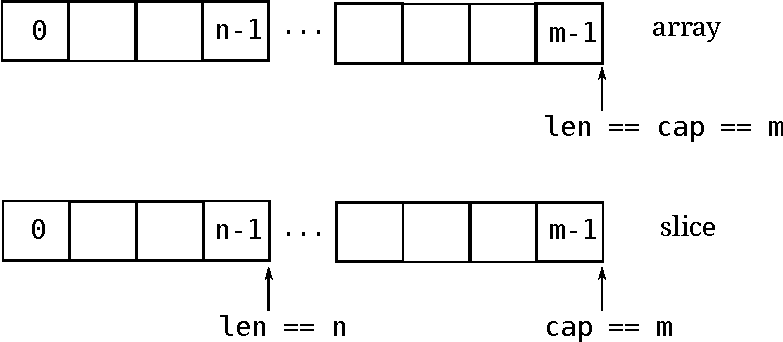
\includegraphics[scale=0.65]{fig/array-vs-slice.pdf}
\end{center}
\end{figure}
Figure \ref{fig:array-vs-slice} depicts the following Go code.
First we create an array of $m$ elements of the type \lstinline{int}:
\lstinline{var array[m+1]int}\newline
Next, we create a slice from this array:
\lstinline{slice := array[0:n+1]}\newline
And now we have:
\begin{itemize}
\item{\lstinline{len(slice) = n, cap(slice) = m}{} ;}
\item{\lstinline{len(array) = cap(array) = m}{} .}
\end{itemize}
The following code defines an array and slice:
\lstinputlisting[numbers=right,label=src:arrays,caption=Arrays and slices]{src/array-and-slices.go}
On line 8 we dare to do to impossible and try to allocate something
beyond the capacity (maximum length of the under laying array) and
we are greeted with a \emph{runtime} error.

\subsection{Maps}
\label{sec:maps}
A lot of other languages have a simular type built-in, Perl has hashes
and Python has got its dictionaries for instance. In Go was have the
\type{map} type. A \type{map} can be thought of as an array indexed by
strings (in its most simple form).
In the following listing we define a \type{map} which converts from a
\lstinline{string} (month abbreviation) to an \lstinline{int} -- the number of days in that month. 
The generic way to define a map is with: \verb|map[<from type>]<to type>|

\begin{lstlisting}
monthdays := map[string]int{
	"Jan": 31, "Feb": 28, "Mar": 31, 
	"Apr": 30, "May": 31, "Jun": 30, 
	"Jul": 31, "Aug": 31, "Sep": 30, 
	"Oct": 31, "Nov": 30, "Dec": 31, |\coderemark{the comma here is OK}|
}		    
\end{lstlisting}
Indexing a map goes like this, suppose we want to print the
number of days in December: \lstinline{fmt.Printf("%d\n", monthdays["Dec"])}\newline
If you're looping over an array, slice, string, or map a \key{range}
clause help you again, which returns the key and corresponding value
with each invocation.
\begin{lstlisting}
year := 0
for _, days := range monthdays  // key is unused
    year += days
}
fmt.Printf("Numbers of days in a year: %d\n", year)
\end{lstlisting}

%% structures

\section{Exercises}
\begin{Exercise}[title={For-loop},difficulty=1]
\label{ex:for-loop}
\Question \label{ex:for-loop q1} Create a simple loop with the \key{for} construct. Make it loop
10 times and print out the loop counter with the \package{fmt} package.

\Question \label{ex:for-loop q2} Put the body of the loop in a separate function.

\Question \label{ex:for-loop q3} Rewrite the loop from 1. to use \key{goto}. The
keyword \key{for} may not be used.
\end{Exercise}

\begin{Answer}

\Question There are a multitude of possibilities, 
one of the solutions could be:
\lstinputlisting[label=src:for,caption=Simple for-loop]{ex-basics/src/for.go}
Lets compile this on an Intel 386 Linux machine and look at the
output.
\vskip\baselineskip
\begin{display}
\pr 8g for.go && 8l -o for for.8
\pr ./for
0
1
.
.
.
9
\end{display}
\vskip\baselineskip

\Question Next we put the body of the 
loop - the \key{fmt.Printf} - in a separate function.
\lstinputlisting[label=src:for-func,caption=Loop calls function]{ex-basics/src/for-func.go}
The presented program should be self explanatory. Note however the
"\lstinline{j int}" instead of the more usual "\lstinline{int j}" in the
function definition.
\end{Answer}


\begin{Exercise}[title={FizzBuzz},difficulty=1]
\label{ex:fizzbuzz}
\Question \label{ex:fizzbuzz q1} Solve this problem, called
the Fizz-Buzz \cite{fizzbuzz} problem:
\begin{quote}
Write a program that prints the numbers from 1 to 100. But for multiples
of three print ``Fizz'' instead of the number and for the multiples of
five print ``Buzz''. For numbers which are multiples of both three and
five print ``FizzBuzz''.
\end{quote}
\end{Exercise}

\begin{Answer}
\Question A possible
solution to this simple problem is the following program.
\lstinputlisting[label=src:fizzbuzz,caption=Fizz-Buzz]{ex-basics/src/fizzbuzz.go}
\showremarks
\end{Answer}


\begin{Exercise}[title={Strings},difficulty=1]
\label{ex:strings}
\Question \label{ex:strings q1} Create a Go program that prints
the following (up to 100 characters):
\begin{alltt}
A
AA
AAA
AAAA
AAAAA
AAAAAA
AAAAAAA
\ldots
\end{alltt}


\Question \label{ex:strings q2} Create a program that counts
the numbers of characters/runes in this string:
\begin{alltt}
asSASA ddd dsjkdsjs dk
\end{alltt}
Make it also output the number of bytes in that string.

\Question \label{ex:string q3} Extend the program from
the previous question to replace the three runes at
position 4 with 'abc'.

\end{Exercise}

\begin{Answer}

\Question The following program is an answer to the first question.
\lstinputlisting[label=string1,caption=Strings]{ex-basics/src/string1.go}

\Question To answer this question we need some help of
the \package{string}-package. First we check the documentation
with \prog{godoc strings | less}. When we read the documentation
we notice two functions: \lstinline{func Bytes(s string) []byte} and
\lstinline{func Runes(s string) []int}. Both return values are
almost what we need, namely (\type{slices}) So we return the length of 
them. Putting this together leads to the following program.
\lstinputlisting[label=string2,caption=Runes in strings]{ex-basics/src/string2.go}
\end{Answer}


%% exercise which maps which can be done with current knowledge, just a
%% print or something

\cleardoublepage
\section{Answers}
\shipoutAnswer
